Dans un éditeur l'ajout d'une parenthèse fermante surnuméraire est signalé (mise en surbrillance). La construction d'un vérificateur de parenthèses repose sur l'utilisation de piles.

\begin{figure}[hbt]
	\begin{center}
		\begin{subfigure}[t]{0.32\textwidth}
			\centering
			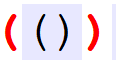
\includegraphics[height=0.2\textwidth]{parentheses/notepadppB}
			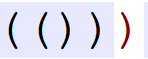
\includegraphics[height=0.2\textwidth]{parentheses/notepadppPB}
			\caption{Éditeur généraliste Notepad++}
		\end{subfigure}
		\hfill
		\begin{subfigure}[t]{0.32\textwidth}
			\centering
			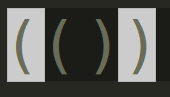
\includegraphics[height=0.2\textwidth]{parentheses/pyzoB}
			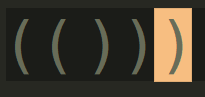
\includegraphics[height=0.2\textwidth]{parentheses/pyzoPB}
			\caption{Éditeur Python Pyzo}
		\end{subfigure}
		\hfill
		\begin{subfigure}[t]{0.32\textwidth}
			\centering
			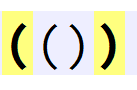
\includegraphics[height=0.2\textwidth]{parentheses/texStudioB}
			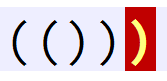
\includegraphics[height=0.2\textwidth]{parentheses/texStudioPB}
			\caption{Éditeur \LaTeX{} TeXstudio}
		\end{subfigure}
		\caption{Expressions bien et mal parenthésées dans différents éditeurs}
	\end{center}
\end{figure}

Nous allons considérer 3 types de ponctuations symétriques~: 
\begin{itemize}
	\item les parenthèses \texttt{(} et \texttt{)}~; 
	\item les crochets \texttt{[} et \texttt{]}~; 
	\item les accolades \texttt{\{} et \texttt{\}}~; 
\end{itemize}

On souhaite savoir reconnaitre 4 cas différents~: 
\begin{itemize}
	\item fermeture sans ouverture préalable~; 
	\item fermeture par le mauvais type de parenthèse~; 
	\item une ouverture sans fermeture~; 
	\item l'expression est bien parenthésée. 
\end{itemize}

Nous allons commencer par nous occuper dans un premier temps uniquement d'un seul type de ponctuations~: les parenthèses. 

\UPSTIquestion Écrire une fonction \texttt{verifPar0(texte)} qui prend en entrée une chaine de caractères et renvoie~: 
\begin{itemize}
	\item le nombre d'ouvertures non-fermées~;
	\item \texttt{-1} dès qu'on rencontre une fermeture sans ouverture préalable.
\end{itemize}
Une pile sera initialisée au début de la fonction~: on ajoutera l'ouverture dans la pile qu'on dépilera lorsqu'il y a fermeture de la parenthèse avec le même type.

\UPSTIquestion Tester la fonction avec \texttt{"(()())"}, \texttt{"(()()"} et \texttt{"(()()))"}.

Nous ajoutons ici les autres types de ponctuations~: il faut donc vérifier si la fermeture correspond bien à l'ouverture dans ce cas-là. 

\UPSTIquestion Écrire une fonction \texttt{verifPar1(texte)} qui prend en entrée une file remplie de caractère et renvoie~: 
\begin{itemize}
	\item le nombre d'ouvertures non-fermées~; 
	\item \texttt{-1} dès qu'on rencontre une fermeture sans ouverture préalable~; 
	\item \texttt{c} dès qu'on rencontre une erreur de type au caractère \texttt{c}.
\end{itemize}

\UPSTIquestion Tester la fonction avec \texttt{"\{[()\}"}, \texttt{"\{[()]"} et \texttt{"\{[()]\}"}.
